% Template for Cogsci submission with R Markdown

% Stuff changed from original Markdown PLOS Template
\documentclass[10pt, letterpaper]{article}

\usepackage{cogsci}


\title{Idiosyncratic but not opaque: Conventions formed in reference
games are interpretable by naïve humans and vision--language models}

\usepackage{booktabs}

\author{{\large \bf Veronica Boyce (vboyce@stanford.edu)} \\ Department of Psychology \\ Stanford University \And {\large \bf Ben Prystawski (benpry@stanford.edu)} \\Department of Psychology \\ Stanford University \AND {\large \bf Alvin Wei Ming Tan (tanawm@stanford.edu)} \\ Department of Psychology \\ Stanford University \And {\large \bf Michael C. Frank (mcfrank@stanford.edu)} \\ Department of Psychology \\ Stanford University}


\begin{document}

\maketitle

\begin{abstract}
In-group linguistic conventions vary in whether they are opaque to
outsiders (teen slang like ``rizz'') or understandable to outsiders
(regionalisms like ``roundabout''). The formation of temporary
linguistic conventions between individuals is often studied in iterated
reference games, where over repeated reference to the same targets, a
describer--matcher pair establishes partner-specific shorthand names for
targets. One open question is how understandable these referring
expressions are to others who were not part of the convention formation
process. We use computational models and experiments with naïve matchers
to assess the opacity of descriptions from iterated reference games.
Both human matchers and the computational model are well above chance
accuracy, suggesting that the conventions substantially reflect aspects
of shared semantic associations. This additional perspective provides
insights into how convention formation relates to models of lexical
uncertainty and efficiency. {[}TODO THIS LAST SENTENCE STILL SUCKS,
please someone fix; 137/150 words atm{]}

\textbf{Keywords:}
reference games; convention formation; computational modeling; opacity;
pragmatics
\end{abstract}

TODO SLIM DOWN INTRO -- target 1.5 pages

TODO should we just drop the efficiency angle? (for space reasons?)

\section{Introduction}\label{introduction}

``He's got rizz.'' The idea that teen slang is arbitrary and opaque to
outsiders (i.e.~older generations) is enough of a cultural touchstone
that late night comedy shows have segments about it. Teens are far from
the only groups that form naming conventions that are specific to the
in-group. Many groups form temporally stable conventions shared by
communities, including professional jargon, regionalisms, and of course
slang. In-group language can be temporally stable conventions shared by
sizable communities, but temporary naming conventions can arise in
smaller groups to refer to a particular entity that doesn't have a label
or even to refer back to group in-jokes.

This formation of temporary linguistic conventions between individuals
is often studied in iterated reference games. In these games, a
describer tells their partner how to sort or match a series of abstract
images (e.g., Clark \& Wilkes-Gibbs, 1986; Hawkins et al., 2020). Over
repeated rounds of referring to the same targets, pairs usually develop
conventionalized nicknames for the target images. These nicknames are
often partner-specific, in that different pairs develop different
nicknames for the same targets. When describing the shapes for people
who were not part of the group, people return to more elaborated
descriptions, indicating an expectation that others may be unable to
understand the convention, and need a longer or different referential
description (Hawkins, Liu, et al., 2021; Wilkes-Gibbs \& Clark, 1992;
Yoon \& Brown-Schmidt, 2018).

In one-shot interactions, the choice of how to map a referring
expression to a target can be modeled using Bayesian pragmatics models
such as Rational Speech Acts model {[}cite{]} that assume speakers and
listeners reasoning about each other. {[}? cite examples of where this
has been used in oneshot ref games{]} Building on these models for
one-shot interactions, the Continual Hierarchical Adaptation through
Inference model (CHAI) introduces partner-specific update rules to allow
for updates to the lexicon after each interaction, which can account for
the shortening of referring expressions observed in games {[}cite{]}.
Initially, speakers have uncertainty about the listeners word-meaning
mappings (lexicon) and so may use multiple words to triangulate a
meaning, but when that succeeds, the updating then leads the agent to be
able to successfully use individual words for the same meaning as the
word-meaning association has been strengthened.

In models like CHAI, both speaker and listener agents are jointly
reasoning about each other, but the same types of models can be used
when the interaction is one-sided. How can listeners understand speakers
when they don't know the semantic lexicon of the speaker? Following
Bayesian approaches to pragmatics and communication, one approach is to
model listeners as Bayesian agents who jointly infer the meaning of a
speaker's utterance and their model of the speaker's lexicon. This
Bayesian joint updating has been used to model word learning, but also
to model person-to-person or group-to-group differences in lexicon
{[}citations TODO{]}. Notably, lexical uncertainty models can account
for times when a listener infers non-shared aspects of the speaker's
lexicon. Often this doesn't mean learning totally arbitrary meaning to
word mappings for each possible interlocutor, but more like learning a
hierarchical set of modifications to a lexicon where some words have
slightly different extensions for different speakers and different
circumstances (Hawkins, Franke, et al., 2021; Schuster \& Degen, 2020).
However, in some experimental settings, people can even learn
contronymic mappings, where the same symbol has context-dependent
opposite meanings (Misyak et al., 2016).

When groups of people form conventions, are they generally opaque to
outsiders (like ``rizz'') or are they generally inferable using some
lexical uncertainty (like ``roundabout'')? {[}is ``rotary'' more
obscure? maybe switch?{]} Iterated reference games provide a controlled
test environment for studying convention formation where the pressures
driving convention formation are purely communicative. Thus, they
provide a test case for studying to what extent opacity is an inherent
consequence of convention formation, or whether it is a separate
sociolinguistic effect for marking in-groupness. Conventions in iterated
reference games are formed between people without a (known) shared group
identity prior to the interaction, but, as seen in partner-switch
experiments, people do not use the conventions with new partners. Do
temporary conventions formed out of communicative need reflect overall
semantic properties, or are they arbitrary in a way that requires one to
``have been there''? One way to operationalize whether term -- meaning
alignments are random or reflective of small deviations from the shared
lexicon is to look at the semantic distance between the signifier and
the referent in semantic space. Expressions that are more transparent
are those where signifiers and referents that are semantically close,
such that any member of the language community sharing the global
semantics should be able to identify the appropriate referent given the
signifier. In contrast, expressions that are opaque have signifiers and
referents that are semantically distant, such that the relations between
them are more arbitrary and inaccessible to the general community
without the formation of additional conventions (which may be partner-
or group-specific).

How can we measure the semantic distances between a conventionalized
referring expression and its target referent? One computational option
is to use vision-language models as a way to operationalize a shared
semantic space for both language and target image. Computational methods
have enabled the embedding of various stimuli (including images and
text) into high-dimensional feature spaces; these embeddings have
properties which suggest that they are reasonable approximations of
humans' semantic spaces, including similarity in representational
geometries (e.g., Grand et al., 2022; Muttenthaler \& Hebart, 2021).
Indeed, embeddings from neural network models have been used as a form
of semantics in a range of reference game scenarios (e.g., Gul \& Artzi,
2024; Ji et al., 2022; Kang et al., 2020; Le et al., 2022; Ohmer et al.,
2022). In particular, such embeddings can be treated as the default
context- and speaker-independent lexicon, since they are not updated to
account for convention formation within an iterated reference game.

An alternative way of measuring the transparency of conventionalized
referring expressions is to directly measure how often naive humans, who
were not part of the group who formed the convention, can correctly
select the target referent given the referring expression. Prior work
with naive matchers has focused on the role of conversational shared
history as an aid to understanding later, more conventionalized
descriptions. Overall, naive matchers tend to do better the more their
observation history resembles that of the original conversation. Naive
listeners in Murfitt \& McAllister (2001) did better when they heard
descriptions in order instead of in reverse order. Schober \& Clark
(1989) found that matchers in an iterated reference game achieved higher
accuracies than overhearers who listened to the entire game in order,
and overhearers who listened to recordings starting in the third round
did even worse. In an iterated reference game using drawing as the
communication modality, Hawkins et al. (2023) found that yoked matchers
who saw all the trials from one game in order outperformed shuffled
matchers who saw trials sampled from 10 games but in trial order.

Across the prior literature, while naïve matchers have worse accuracy
than in-game matchers, their performance was still far above chance,
suggesting that the convention--target relationship is not purely
arbitrary. In fact, even when pairs of participants try to obfuscate
their meaning to match images with each other but not an overhearer, an
overhearing participant can still do quite well (Clark \& Schaefer,
1987). Nonetheless, receiving more context from an interaction---and in
particular, having that context be in order---is beneficial to matchers.
Except for the shuffled condition of Hawkins et al. (2023), these
studies do not address how opaque descriptions from different points in
the game are without prior context. Such an approach would be important
to have truly naïve matchers that lack even the context of trial order,
providing a clearer understanding of when these expressions are opaque
and when they are merely idiosyncratic.

In the current work, we address how the process of convention formation
shapes the levels of opacity of the referring expressions created at
different time points in an iterated reference game. We draw our
reference game expressions from Boyce et al. (2024), which has a large
corpus of iterated reference games played by groups of different sizes,
all playing online and communicating via a chat box. This corpus is made
up of 6-round iterated reference games using the same 12 target images.
Games were played in conditions varying in how large the
describer--matcher groups were (2--6 participants) and how ``thick'' the
communication channels were. The varied conditions within a consistent
framework allow us to test how opacity of referring expressions vary
depending on the conditions they were produced under.

Using reference expressions created in different games from Boyce et al.
(2024), we use both human experiments and models to assess when and why
expressions are opaque or understandable to outside observers. We first
present a computational approach using a vision-language model with a
read-out head to determine the semantic similarities between referring
expressions and their targets and validate against naive human matchers
(Experiment 1). We compare the opacity referring expressions across
different game conditions and time points using both naive human
matchers and the model (Experiment 2). Finally, we address the role of
conversation history by comparing human matcher performance on shuffled
versus ordered game transcripts (Experiment 3).

\begin{CodeChunk}
\begin{figure}[t!]

{\centering 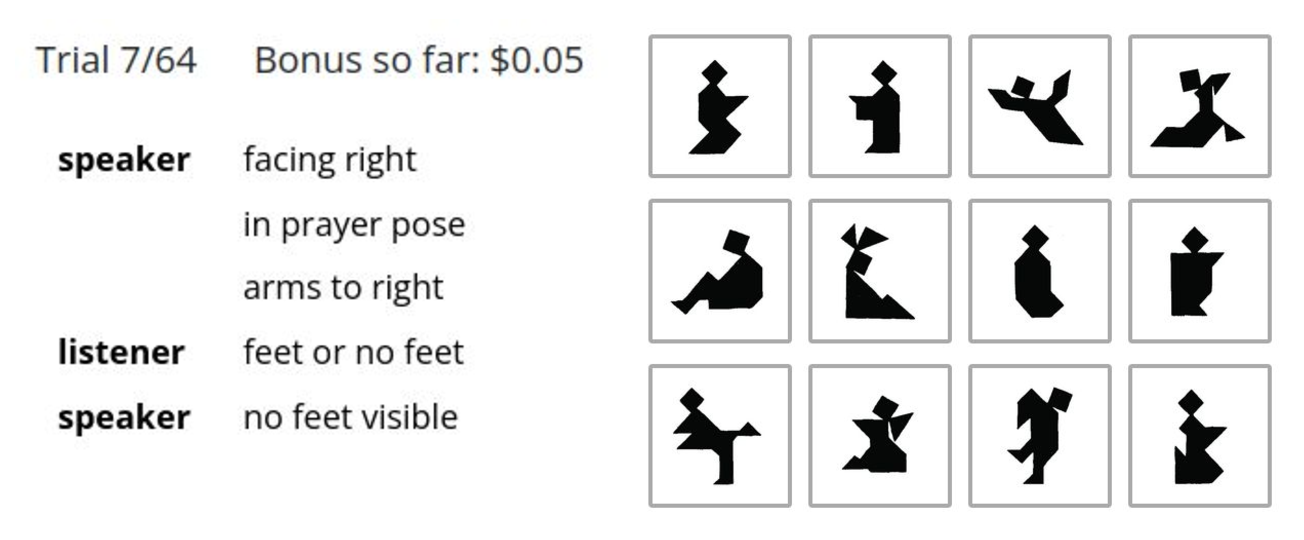
\includegraphics[width=1\linewidth]{matcher-diagram} 

}

\caption[Experimental Setup]{Experimental Setup. Naive matchers read transcripts from trials in reference games from Boyce et al. (2024) and selected which image they thought was being described. Matchers recieved bonus payments for correct selections. \label{game}}\label{fig:interface}
\end{figure}
\end{CodeChunk}

\section{Task setup}\label{task-setup}

\subsection{Materials}\label{materials}

We drew our referential expressions from Boyce et al. (2024). For our
naïve matcher experiments, we sampled different subsets of this corpus.
In presenting the transcripts, we excluded utterances that were marked
by Boyce et al. (2024) as not containing any referential content. Within
the samples, we also did not show transcripts that contained swear words
or crude or sexual language. We used the entire corpus for our
computational modeling component.

\subsection{Experimental procedure}\label{experimental-procedure}

We recruited English-speaking participants from Prolific. Participants
were directed to the experiment, where the task was explained to them.
On each trial, participants saw the full transcript from that trial,
containing all the chat messages marked by whether they were from the
speaker or a listener. Participants selected the image they thought was
the target from the tableau of 12 (Figure \ref{game}). Participants
received feedback on whether they were right or wrong on each trial.
Except when the specific viewing order was part of the experimental
manipulation, we randomized the order of trials, subject to the
constraint that the same target could not repeat on adjacent trials. The
task was implemented in jsPsych (Leeuw et al., 2023). We paid
participants \$10 an hour plus a bonus of 5 cents per correct response.
All our experimental code is at TODO OSF LINK GOES HERE.

\subsection{Computational models}\label{computational-models}

We used CLIP (\texttt{clip-vit-large-patch14}) as a listener model for
our domain (Radford et al., 2021) TODO BEN say model architecture/type.
CLIP is a natural choice for reference games, as the model is trained to
estimate the correspondence between images and phrases in natural
language. We pre-processed the text by concatenating all the messages
sent by the speaker for a given trial, and ran CLIP for the concatenated
text and all 12 tangram shapes. We then computed probabilities for each
tangram shape using CLIP's logits. The simplest way to do this is simply
taking the softmax of the logits. However, the tangram shapes were
possibly out the distribution for the model, which led it to favor some
images over others regardless of the content of the text. To fix this,
we trained readout models that made more calibrated predictions using
CLIP's logits.

\begin{table}
\caption{Cross-validated accuracies for classifiers. Standard deviations in accuracy across the 10 folds are shown in parentheses. Best performance within each model class is underlined, and best overall performance is bolded.}
\label{tab:classifier_comparison}
\centering

  \begin{tabular}{p{1em}lr}
    \toprule
    \multicolumn{2}{l}{Classifier} & Accuracy \\ 
    \midrule
        \multicolumn{2}{l}{Random baseline} & \smash{0.08} \\
    \multicolumn{2}{l}{CLIP without readout} & \smash{0.31} \\
    \multicolumn{2}{l}{Logistic regression} & \\
    & No penalty & \underline{\smash{0.50 (0.01)}} \\ 
    & \vspace{1mm}L2 penalty & 0.50  (0.01) \\ 
    \multicolumn{2}{l}{Random forest} & \\
    & 10 estimators & 0.46 (0.02) \\
    & 50 estimators  & 0.51 (0.02)\\ 
    & 100 estimators & 0.52 (0.02) \\ 
    & \vspace{1mm}500 estimators & \underline{\smash{0.52 (0.02)}} \\ 
    \multicolumn{2}{l}{Gradient-boosted tree} & \\
    & 10 estimators & 0.48 (0.02) \\ 
    & \vspace{1mm}100 estimators & \underline{\smash{0.51 (0.02)}} \\ 
    \multicolumn{2}{l}{Multi-layer perceptron} & \\
    & 1 $\times$ 32-dim hidden layer & 0.50 (0.01) \\ 
    & 1 $\times$ 100-dim hidden layer  & 0.52 (0.01) \\ 
    & 1 $\times$ 512-dim hidden layer & 0.53 (0.02) \\ 
    & 1 $\times$ 1028-dim hidden layer & 0.53 (0.02) \\ 
    & 2 $\times$ 32-dim hidden layers  & 0.51 (0.02) \\ 
    & 2 $\times$ 100-dim hidden layers & \underline{\smash{\textbf{0.55 (0.02)}}} \\ 
    \bottomrule
    \end{tabular}
\end{table}

We trained different readout models to assign probabilities to features
using CLIP's logits as features. Models were trained to maximize task
performance (i.e., to assign high probability to the target tangram
given the concatenated speaker utterance). We compared four types of
models: a random forest, a logistic regression model, a multi-layer
perceptron (MLP), and a gradient-boosted tree. Classifiers were
implemented in the \texttt{scikit-learn} and \texttt{XGBoost} libraries
(Chen \& Guestrin, 2016; Pedregosa et al., 2011). Table
\ref{tab:classifier_comparison} shows the cross-validated accuracy of
different readout models, as well as the performance of CLIP with no
readout. The MLP with two hidden layers of size 100 performed the best,
so we use its predictions in subsequent analysis. TODO BEN clarify when
things are held out v not!

\section{Experiment 1}\label{experiment-1}

\begin{CodeChunk}
\begin{figure}[t]

{\centering 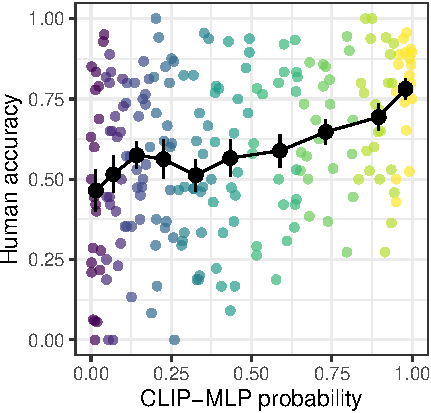
\includegraphics[width=0.7\linewidth]{figs/fig-calibration-1} 

}

\caption[Correlation between human accuracy and CLIP-MLP probability of target in Experiment 1]{Correlation between human accuracy and CLIP-MLP probability of target in Experiment 1.  Points are individual descriptions, colored by decile of CLIP-MLP probability, black line is the bootstrapped mean and 95\% CI across descriptions for each decile. \label{calibration}}\label{fig:fig-calibration}
\end{figure}
\end{CodeChunk}

Our CLIP-MLP computational model was optimized for task accuracy. To
validate whether this objective also results in human-like response
patterns, we conducted a calibration experiment to determine if, for any
given utterance, the model-assigned target probability was aligned with
the probability that a naïve human matcher would choose the target
image.

\subsection{Methods}\label{methods}

We first obtained target probabilities from our CLIP-MLP model for all
utterances from Boyce et al. (2024). We then used stratified sampling to
select 217 trials by dividing model-predicted probabilities into deciles
and choosing approximately 22 utterances per decile, spanning the 12
different possible target images. We recruited 61 participants who each
saw 64 trials randomly sampled from the 217 tested trials. On average,
each trial was seen by 18 participants. This experiment was
pre-registered at \url{https://osf.io/6pv5e}.

\subsection{Results and discussion}\label{results-and-discussion}

We obtained human accuracies on each trial by dividing the number of
participants who selected the target by the total number of participants
who saw the trial (Figure \ref{fig:fig-calibration}). There was a modest
but significant positive correlation between model-predicted
probabilities and human accuracies (\(r\) = 0.33 {[}0.21, 0.45{]}). This
result suggests that model predictions were calibrated to human response
patterns, albeit not perfectly. It is possible to use these calibration
results to tune model predictions to better approximate human responses;
we leave this approach for future work. Nonetheless, the observed
positive correlation suggests that our computational model carries some
signal about human accuracies, validating its use in subsequent
experiments as a computational comparison.

\begin{CodeChunk}
\begin{figure}[t]

{\centering 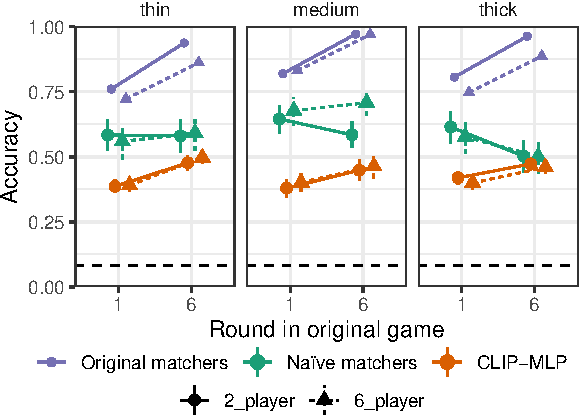
\includegraphics[width=0.9\linewidth]{figs/fig-condition-1} 

}

\caption[Accuracies for naïve human matchers and the CLIP-MLP model for Experiments 2a and 2b, grouped by the source of the referential description]{Accuracies for naïve human matchers and the CLIP-MLP model for Experiments 2a and 2b, grouped by the source of the referential description. Facets are the communication thickness of the original game and x-axis is when in the game the transcript caome form. Point estimates and 95\% CrI are predictions from the fixed effects of logistic and beta regressions. Bootstrapped mean accuracy from the original matchers is included as a ceiling, and random chance as a baseline. \label{expt2-condition}}\label{fig:fig-condition}
\end{figure}
\end{CodeChunk}

\begin{CodeChunk}
\begin{figure}[t]

{\centering 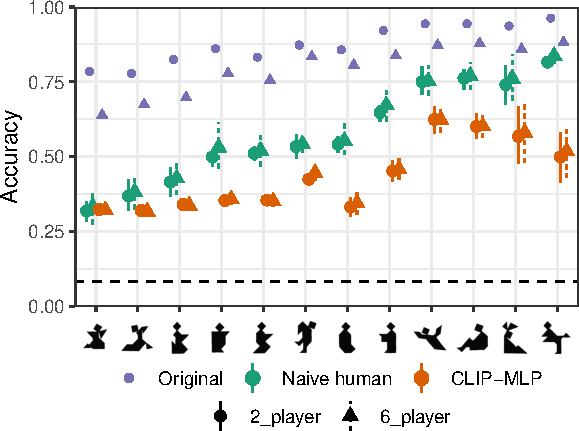
\includegraphics[width=0.9\linewidth]{figs/fig-2-1} 

}

\caption[Accuracies for naïve human matchers and the CLIP-MLP model for Experiments 2a and 2b, split out by target image]{Accuracies for naïve human matchers and the CLIP-MLP model for Experiments 2a and 2b, split out by target image. Point estimates and 95\% CI are predictions from the fixed effects and by-tangram random effects of logistic and beta regressions, bootstrapped across conditions. Bootstrapped mean accuracy from the original matchers is included as a ceiling, and random chance as a baseline. \label{expt2-tangram}}\label{fig:fig-2}
\end{figure}
\end{CodeChunk}

\section{Experiment 2}\label{experiment-2}

As a starting point for examining what makes referential expressions
more or less opaque, we focused on referring expressions from the first
and last rounds of games. Principles of convention formation and
people's behavior when switching to a new partner suggest that
later-round utterances are more opaque and thus harder to understand.
One counterargument is that later rounds are the result of describers'
accumulated practice refining descriptions to be maximally communicative
and to pick out the most visually salient features. To distinguish these
hypotheses, we ran a recognition experiment including descriptions from
games of different sizes and communication thicknesses. Based on the
patterns of cross-game similarity in Boyce et al. (2024), we expected
that smaller and thicker games, whose descriptions diverged fastest,
would have more idiosyncratic and opaque conventions than larger groups
with thinner communication channels.

\subsection{Methods}\label{methods-1}

\subsubsection{Experiment 2a}\label{experiment-2a}

To establish a baseline of how well naïve matchers could understand
descriptions without context, we ran a 2x2 within subjects experiment.
We drew the target transcripts from 2- and 6-player games from
Experiment 1 of Boyce et al. (2024) and from the first and last blocks
of these games. These games had medium-thick communication channels,
where matchers could send text messages to the shared chat interface,
but the describer role rotated each round, and matchers received limited
feedback. We recruited 60 participants who each saw 60 trials (15 in
each of the 4 conditions). Overall, participants saw 774 transcripts
from 40 games. This experiment was pre-registered at
\url{https://osf.io/k45dr}.

\subsubsection{Experiment 2b}\label{experiment-2b}

After observing limited condition differences in Experiment 2a, we ran a
follow-up experiment on descriptions from Experiment 3 of Boyce et al.
(2024), where the communication channel thicknesses were more extreme.
Here, we used a 2x2x2 within subjects design, drawing our transcripts
from the first and last rounds of thick and thin, 2- and 6- person
games. In the ``thick'' condition, matchers could send text messages to
the shared chat interface, one person was the the describer role the
whole game, and matchers recived feedback on everyone's selections. In
contrast, in the ``thin'' condition, original matchers could only
contribute to the chat by sending one of 4 emojis, the describer role
rotated, and matchers recieved limited feedback. As the emojis did not
have referential content, we did not include them in the transcripts
shown to naïve matchers. For experiment 2b, we recruited 60 participants
who each saw 64 trials (8 in each of the 8 conditions). Overall,
participants saw 2392 transcripts from 163 games. This experiment was
pre-registered at \url{https://osf.io/rdp5k}.

\subsection{Results}\label{results}

\subsubsection{Experiment 2a}\label{experiment-2a-1}

For Experiment 2a, we ran a Bayesian mixed effects logistic model of
naïve matcher accuracy in brms (Bürkner, 2018).\footnote{correct
  \({\sim}\) group\_size \({\times}\) round~\({+}\) trial\_order~\({+}\)
  (group\_size \({\times}\) round\textbar correct\_tangram)~\({+}\)
  (group\_size \({\times}\) round~\({+}\) trial\_order\textbar workerid)}
Overall, naïve matchers were right 62\% of the time, which was far above
the 1/12 = 8.3\% expected by random chance (OR = 1.93 {[}1.05, 3.62{]}).
There were not large effects of condition (Figure \ref{expt2-condition}
middle panel). Participants tended to be less accurate at descriptions
from the last round (OR of last round = 0.77 {[}0.53, 1.10{]}). There
was not a clear effect of original group size (OR of 6-player game =
1.15 {[}0.89, 1.47{]}), but there was an interaction between round and
group size (OR = 1.49 {[}1.06, 2.10{]}). Later transcripts from larger
games were easier to understand, but earlier transcripts from smaller
games were easier to understand. Much of the variation in accuracy was
driven by the target image, which accounted for more variation than
participant differences (standard deviation of image distribution = 0.98
{[}0.63, 1.51{]}; SD of participant distribution = 0.64 {[}0.42,
0.88{]}). Some images were much easier to identify as the target than
others (Figure \ref{expt2-tangram}).

\subsubsection{Experiment 2b}\label{experiment-2b-1}

For Experiment 2b we ran a similar Bayesian mixed effects logistic
model.\footnote{correct \({\sim}\) group\_size \({\times}\) thickness
  \({\times}\) round~\({+}\) trial\_order~\({+}\) (group\_size
  \({\times}\) thickness \({\times}\)
  round\textbar correct\_tangram)~\({+}\) (group\_size \({\times}\)
  thickness \({\times}\) round~\({+}\) trial\_order\textbar workerid)}
Naïve matchers were above chance (OR = 1.81 {[}1.06, 3.08{]}, Figure
\ref{expt2-condition} ). Similar to experiment 2a, there were not
substantial effects of condition. Last round descriptions had slightly
lower accuracy (OR of last round = 0.64 {[}0.47, 0.85{]}), but there was
an interaction with thickness, where for thin games, last round
descriptions were less opaque (OR = 1.55 {[}1.02, 2.33{]}). Again some
of the uncertainty in estimating the fixed effects was driven by the
strong variation based on target image (0.81 {[}0.51, 1.28{]}), which
again exceeded participant variation (0.62 {[}0.43, 0.83{]}).

\subsubsection{Additional predictors}\label{additional-predictors}

As additional post-hoc predictors, we examined the accuracy of the
in-game matchers from Boyce et al. (2024) and the length of the
description. In both experiments, in-game accuracy was predictive of
naïve matcher accuracy (Expt 2a OR = 3.33 {[}2.45, 4.53{]}, Expt 2b OR =
2.39 {[}1.88, 3.03{]}). The log number of words in the description was
not predictive in Experiment 2a (OR = 1.05 {[}0.94, 1.17{]}), but longer
descriptions were slightly beneficial in Experiment 2b (OR = 1.10
{[}1.01, 1.20{]}).

The pattern of results for when conventions became more opaque was
similar to the pattern of which game conditions produced descriptions
that diverged the most in semantic space in Boyce et al. (2024). As a
post-hoc test of whether opacity might be related to semantic
divergence, we used the mean semantic similarity between an utterance
and other utterances in the same condition as an additional predictor of
accuracy.\footnote{Semantic similarity was operationalized as cosine
  similarity between S-BERT embeddings (\textbf{reimers2019?}), the
  measure of semantic distance used in Boyce et al. (2024).} Similarity
to other utterances was strongly predictive of increased accuracy in
both experiments (Expt 2a: OR = 12.49 {[}4.70, 33.64{]}, Expt 2b: OR =
14.75 {[}5.93, 36.87{]}) and was more predictive for the last round
descriptions (Expt 2a: OR = 3.49 {[}1.09, 10.92{]}, Expt 2b: OR = 4.78
{[}1.61, 14.25{]}). While exploratory, this analysis suggests that
referring expressions that are further from shared semantic priors are
harder for naive listeners to understand.

\subsection{Model results}\label{model-results}

As a computational comparison, we looked at the CLIP-MLP model's
performance on the same descriptions. We used the probability the model
assigned to the correct target as our dependent measure and fit a
Bayesian mixed effects beta regression on the descriptions from
Experiment 2.\footnote{correct \({\sim}\) group\_size \({\times}\)
  thickness \({\times}\) round~\({+}\) (group\_size \({\times}\)
  thickness \({\times}\) round\textbar correct\_tangram)} The CLIP-MLP
model was far above chance, but had lower accuracy than the human
participants (OR = 0.60 {[}0.45, 0.82{]}). The strongest predictor of
accuracy was later round (OR = roundround\_6: 1.32 {[}0.94, 1.83{]}),
but even this was uncertain. There was substantial by-target image
variation (0.46 {[}0.27, 0.76{]}).

In additional models, we checked the effect of in-game matcher accuracy,
length of the description, and semantic divergence. CLIP-MLP had higher
accuracy when in-game matcher accuracy was higher (OR = 1.52 {[}1.35,
1.71{]}), and the model did better on shorter descriptions (OR for log
words = 0.85 {[}0.82, 0.90{]}). Long descriptions may be difficult
because they are further further from the model's training distribution
of image captions. Semantic similarity to other descriptions from the
same type of games was predictive of higher accuracy (OR = 11.85
{[}6.51, 21.06{]}), especially for last round utterances (OR = 3.46
{[}1.65, 7.36{]}).

\subsection{Discussion}\label{discussion}

Overall, naïve human matchers were fairly accurate overall, but less
accurate than matchers in the original game. The computational model was
less accurate, but still far above chance. The largest source of
variability in accuracy was from target images, and whether earlier or
later utterances were more opaque varied by game condition. While not a
pre-planned analysis, the level of semantic divergence from other
expressions was strongly predictive of the opacity of the expression
(for both humans and the model), suggesting that descriptions that were
closer to shared semantic priors were more transparent.

\section{Experiment 3}\label{experiment-3}

The experiment of naïve matchers in Experiment 2 differed from in-game
matchers in several ways. In-game matchers recieved descriptions from a
consistent group, recieved descriptions in the order they were created,
and were present participants during the game. In Experiment 3, we
focused on the role of context and group-specific interaction history to
tease apart some of these differences. Our primary question of interest
was how much seeing the entire the conversation history in order would
help participants understand later round descriptions.

\subsection{Methods}\label{methods-2}

We compared naïve matchers in ``yoked'' and ``shuffled'' conditions. In
the ``yoked'' condition, naïve matchers saw all the descriptions from a
single game in the order they originally occurred. In the ``shuffled''
condition, naïve matchers saw all the descriptions from a single game in
a randomized order. This is the same yoking but a different shuffling
than that used in Hawkins et al. (2023).

Because some descriptions are already fairly comprehensible in
isolation, we focused on games that showed strong group-specificity. We
hand-picked 10 games from Boyce et al. (2024) on the basis of high
in-game matcher accuracy, strong patterns of descriptions shortening
over repetition, and the use of idiosyncratic or non-modal referring
expressions. Thus, these games showed the hallmarks of strong
conventionalization to terms that were more likely to be opaque to
outsiders.

We recruited 196 participants (99 in the yoked condition and 97 in
shuffled) who each saw all 72 trials of one of the 10 games. This
experiment was pre-registered at \url{https://osf.io/zqwp5}.
Participants read the transcripts in a modified self-paced reading
procedure where they uncovered the text word by word (revealed words
stayed visible); only after uncovering the entire transcript could
participants select an image. We do not analyze the reading time data
here.

\begin{CodeChunk}
\begin{figure}[t]

{\centering 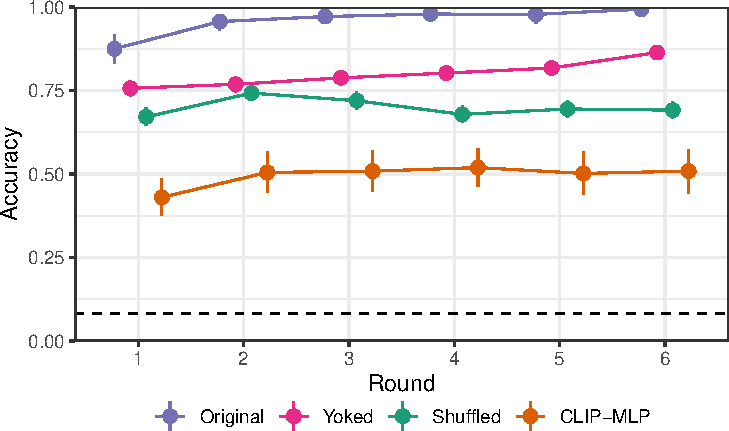
\includegraphics[width=0.9\linewidth]{figs/fig-yoked-1} 

}

\caption[Accuracies for Experiment 3]{Accuracies for Experiment 3. Error bars are bootstrapped 95\% CIs. TODO not using predictions because those fuzz out round to round differences. \label{yoked}}\label{fig:fig-yoked}
\end{figure}
\end{CodeChunk}

\subsection{Results and discussion}\label{results-and-discussion-1}

Our primary question of interest was how much seeing the conversation
history unfold in order would help participants interpret descriptions,
especially those from later rounds after conventions had formed.

We compared accuracy across the yoked and shuffled conditions with a
Bayesian mixed effects logistic regression.\footnote{correct \({\sim}\)
  orig\_repNum \({\times}\) condition~\({+}\) matcher\_trialNum~\({+}\)
  (1\textbar gameId)~\({+}\) (1\textbar correct\_tangram)~\({+}\)
  (1\textbar workerid)}. The descriptions were more transparent when
they were presented in a yoked order (OR = 2.20 {[}1.63, 3.00{]}, Figure
\ref{yoked}). In the shuffled condition, there was no main effect of
round number (OR for one round later = 0.99 {[}0.95, 1.02{]}), but there
was a marginal interaction where the benefit of the yoked condition
decreased for later rounds (OR for one round later = 0.94 {[}0.89,
1.00{]}). This was offset by matchers in both conditions improving at
the task over time (OR for one trial later in matcher viewing order =
1.02 {[}1.02, 1.02{]}). In the yoked condition round and trial number
were aligned, so an improvement over time could be either from matcher
practice or from descriptions being easier to understand. In the
shuffled condition, matcher practice effects did not correlate with
position in the original game.

Comparing to the performance of in-game matchers, we can separate out
the benefits of seeing the descriptions in order versus being a
participant in the group.\footnote{correct \({\sim}\) orig\_repNum
  \({\times}\) order~\({+}\) orig\_repNum \({\times}\) setting~\({+}\)
  matcher\_trialNum~\({+}\) (1\textbar gameId)~\({+}\)
  (1\textbar correct\_tangram)~\({+}\) (1\textbar workerid)} There is a
benefit to seeing the items in order (OR = 2.24 {[}1.63, 3.04{]}) and a
larger benefit to being a participant during the game (OR = 4.35
{[}2.77, 6.89{]}). The benefit of seeing the items in order wanes in
later blocks (OR = 0.94 {[}0.89, 1.00{]}), but the benefit of being in
the game does not (OR = 1.06 {[}0.95, 1.18{]}). In all cases, there is a
baseline improvement over trials (OR = 1.02 {[}1.02, 1.02{]}).

The accuracy of the CLIP-MLP model is worse than the shuffled human
results, and does not show change across rounds (OR for one round later
= 1.02 {[}0.97, 1.07{]}). The larger difference between naïve human and
CLIP-MLP accuracies in Experiment 3 than Experiment 2 could suggest that
even the shuffled ordering still provides useful context (e.g., the
consistent set of images) that helps matchers understand the
conventions. This history is not available to the CLIP-MLP model which
sees every description as a one-shot task.

\section{General discussion}\label{general-discussion}

Real-world conventions vary in whether they are opaque to outsiders
(``rizz'') or comprehensible even to those who don't produce them
(``roundabout''). Convention formation in the real world is subject to a
number of pressures (including communicative ones and social ones), but
is also difficult to study. As a controlled experimental situation,
iterated reference games provide a way of studying convention formation
driven by communicative needs.

Conventions are formed in reference games in a partner-specific way,
where different groups follow different paths through semantic space as
they form conventions. However, the referential descriptions used over
the course of convention formation remain relatively understandable to
outsiders. Across multiple experiments with human matchers, we found
that naïve human matchers were far above chance accuracy at identifying
the targets, with variation explained more by the target image than the
round or game condition the descriptions came from. Even for games
selected for strong conventionalization, naïve matchers had high
accuracy overall, although this accuracy was increased if they followed
the process of conventionalization and saw utterances in order.

There were suggestive patterns that descriptions that were further from
the norm were more opaque.

We also tested a computational model built on CLIP with a multi-layer
perceptron readout as a way of approximating the context-independent
semantic distance between descriptions and images. The CLIP-MLP model
was far above chance in its assignment of probabilities to target images
and correlated with human accuracies, although its probabilities were
lower than human matcher accuracies.

This work suggests that conventions formed within a small group may
still be fairly comprehensible to those outside the group, who may
produce different descriptions themselves. This finding raises questions
around how well-calibrated describers are to their matcher's level of
knowledge, and whether the process of convention formation is actually
efficient. Even naïve matchers can often understand the shorthand
descriptions, especially when there has not been a lot of semantic
drift, but in reference games, describers choose elaborated descriptions
with new matchers. In a game, norms of cooperation and conversation may
lead describers to start new matchers with elaborated descriptions
designed to give them a high level of confidence in target selection.
Describers are also constrained by their need to come up with a
description in real time. However, the high level of understanding and
the lack of substantial benefit from early round descriptions does raise
empirical questions about how calibrated describers are to the level of
information necessary.

Our experimental and computational results were only on a specific set
of iterated reference game transcripts targeting a specific set of 12
images. There are potential non-measured differences between in-game
matchers and naïve matchers, particularly in terms of effort and time
spent on the task.

Some images may lend themselves to more transparent descriptions because
they are more iconic, with a narrower prior over different ways they
could be conceptualized, or they may be further from competitors within
this pool of images. We are limited by the 12 images we used, but future
work sampling across larger sets of images (such as Ji et al., 2022)
could probe image-level factors. Future work could also explore
within-description sources of variation and how the structure and word
choice of utterance correlates with naïve matcher accuracy.
Computational models could be especially beneficial because they could
be run on subsets or ablations of descriptive text.

A difficulty with scaling up computational models like CHAI and RSA to
be a generative model of natural language reference games is the issue
of how to handle baseline semantics. Even without a generative model,
the lexical uncertainty approach is a useful one for understanding how
information is conveyed and conventions formed in iterated reference
games. It also provide a useful lens for examining flexibility of
semantics and how new meanings arise and are understood. TODO could use
another concluding sentence!

\section{References}\label{references}

\setlength{\parindent}{-0.1in} 
\setlength{\leftskip}{0.125in}

\noindent

\phantomsection\label{refs}
\begin{CSLReferences}{1}{0}
\bibitem[\citeproctext]{ref-boyce2024}
Boyce, V., Hawkins, R., Goodman, N. D., \& Frank, M. C. (2024).
\emph{Interaction structure constrains the emergence of conventions in
group communication}.

\bibitem[\citeproctext]{ref-burkner2018}
Bürkner, P.-C. (2018). Advanced bayesian multilevel modeling with the r
package brms. \emph{The R Journal}, \emph{10}(1), 395--411.

\bibitem[\citeproctext]{ref-chen2016xgboost}
Chen, T., \& Guestrin, C. (2016). Xgboost: {A} scalable tree boosting
system. \emph{Proceedings of the 22nd Acm Sigkdd International
Conference on Knowledge Discovery and Data Mining}, 785--794.

\bibitem[\citeproctext]{ref-clark1987a}
Clark, H. H., \& Schaefer, E. F. (1987). Concealing one's meaning from
overhearers. \emph{Journal of Memory and Language}, \emph{26}(2),
209--225. \url{https://doi.org/10.1016/0749-596X(87)90124-0}

\bibitem[\citeproctext]{ref-clark1986}
Clark, H. H., \& Wilkes-Gibbs, D. (1986). \emph{Referring as a
collaborative process}.

\bibitem[\citeproctext]{ref-grand2022}
Grand, G., Blank, I. A., Pereira, F., \& Fedorenko, E. (2022). Semantic
projection recovers rich human knowledge of multiple object features
from word embeddings. \emph{Nature Human Behaviour}, \emph{6}(7),
975--987. \url{https://doi.org/10.1038/s41562-022-01316-8}

\bibitem[\citeproctext]{ref-gul2024}
Gul, M. O., \& Artzi, Y. (2024). \emph{{CoGen}: {Learning} from
{Feedback} with {Coupled Comprehension} and {Generation}}
(arXiv:2408.15992). arXiv.
\url{https://doi.org/10.48550/arXiv.2408.15992}

\bibitem[\citeproctext]{ref-hawkins2020b}
Hawkins, R. D., Frank, M. C., \& Goodman, N. D. (2020). Characterizing
the dynamics of learning in repeated reference games.
\emph{arXiv:1912.07199 {[}Cs{]}}. \url{https://arxiv.org/abs/1912.07199}

\bibitem[\citeproctext]{ref-hawkins2021a}
Hawkins, R. D., Franke, M., Frank, M. C., Goldberg, A. E., Smith, K.,
Griffiths, T. L., \& Goodman, N. D. (2021). \emph{From partners to
populations: {A} hierarchical {Bayesian} account of coordination and
convention} (arXiv:2104.05857). arXiv.
\url{https://doi.org/10.48550/arXiv.2104.05857}

\bibitem[\citeproctext]{ref-hawkins2021}
Hawkins, R. D., Liu, I., Goldberg, A. E., \& Griffiths, T. G. (2021).
Respect the code: {Speakers} expect novel conventions to generalize
within but not across social group boundaries. \emph{CogSci}.

\bibitem[\citeproctext]{ref-hawkins2023a}
Hawkins, R. D., Sano, M., Goodman, N. D., \& Fan, J. E. (2023). Visual
resemblance and interaction history jointly constrain pictorial meaning.
\emph{Nature Communications}, \emph{14}(1), 2199.
\url{https://doi.org/10.1038/s41467-023-37737-w}

\bibitem[\citeproctext]{ref-ji2022}
Ji, A., Kojima, N., Rush, N., Suhr, A., Vong, W. K., Hawkins, R., \&
Artzi, Y. (2022). Abstract {Visual Reasoning} with {Tangram Shapes}. In
Y. Goldberg, Z. Kozareva, \& Y. Zhang (Eds.), \emph{Proceedings of the
2022 {Conference} on {Empirical Methods} in {Natural Language
Processing}} (pp. 582--601). Association for Computational Linguistics.
\url{https://doi.org/10.18653/v1/2022.emnlp-main.38}

\bibitem[\citeproctext]{ref-kang2020}
Kang, Y., Wang, T., \& de Melo, G. (2020). Incorporating {Pragmatic
Reasoning Communication} into {Emergent Language}. \emph{Advances in
{Neural Information Processing Systems}}, \emph{33}, 10348--10359.

\bibitem[\citeproctext]{ref-le2022}
Le, H., Daryanto, T., Zhafransyah, F., Wijaya, D., Coppock, E., \& Chin,
S. (2022). \emph{Referring {Expressions} with {Rational Speech Act
Framework}: {A Probabilistic Approach}} (arXiv:2205.07795). arXiv.
\url{https://doi.org/10.48550/arXiv.2205.07795}

\bibitem[\citeproctext]{ref-leeuw2023}
Leeuw, J. R. de, Gilbert, R. A., \& Luchterhandt, B. (2023). {jsPsych}:
{Enabling} an {Open-Source Collaborative Ecosystem} of {Behavioral
Experiments}. \emph{Journal of Open Source Software}, \emph{8}(85),
5351. \url{https://doi.org/10.21105/joss.05351}

\bibitem[\citeproctext]{ref-misyak2016}
Misyak, J., Noguchi, T., \& Chater, N. (2016). Instantaneous
{Conventions}: {The Emergence} of {Flexible Communicative Signals}.
\emph{Psychological Science}, \emph{27}(12), 1550--1561.
\url{https://doi.org/10.1177/0956797616661199}

\bibitem[\citeproctext]{ref-murfitt2001}
Murfitt, T., \& McAllister, J. (2001). The {Effect} of {Production
Variables} in {Monolog} and {Dialog} on {Comprehension} by {Novel
Listeners}. \emph{Language and Speech}, \emph{44}(3), 325--350.
\url{https://doi.org/10.1177/00238309010440030201}

\bibitem[\citeproctext]{ref-muttenthaler2021}
Muttenthaler, L., \& Hebart, M. N. (2021). {THINGSvision}: {A Python
Toolbox} for {Streamlining} the {Extraction} of {Activations From Deep
Neural Networks}. \emph{Frontiers in Neuroinformatics}, \emph{15}.
\url{https://doi.org/10.3389/fninf.2021.679838}

\bibitem[\citeproctext]{ref-ohmer2022}
Ohmer, X., Franke, M., \& König, P. (2022). Mutual {Exclusivity} in
{Pragmatic Agents}. \emph{Cognitive Science}, \emph{46}(1), e13069.
\url{https://doi.org/10.1111/cogs.13069}

\bibitem[\citeproctext]{ref-pedregosa2011scikit}
Pedregosa, F., Varoquaux, G., Gramfort, A., Michel, V., Thirion, B.,
Grisel, O., Blondel, M., Prettenhofer, P., Weiss, R., Dubourg, V., et
al. (2011). Scikit-learn: {Machine} learning in python. \emph{The
Journal of Machine Learning Research}, \emph{12}, 2825--2830.

\bibitem[\citeproctext]{ref-radford2021}
Radford, A., Kim, J. W., Hallacy, C., Ramesh, A., Goh, G., Agarwal, S.,
Sastry, G., Askell, A., Mishkin, P., Clark, J., Krueger, G., \&
Sutskever, I. (2021). \emph{Learning {Transferable Visual Models From
Natural Language Supervision}} (arXiv:2103.00020). arXiv.
\url{https://doi.org/10.48550/arXiv.2103.00020}

\bibitem[\citeproctext]{ref-schober1989}
Schober, M. F., \& Clark, H. H. (1989). Understanding by addressees and
overhearers. \emph{Cognitive Psychology}, \emph{21}(2), 211--232.
\url{https://doi.org/10.1016/0010-0285(89)90008-X}

\bibitem[\citeproctext]{ref-schuster2020}
Schuster, S., \& Degen, J. (2020). I know what you're probably going to
say: {Listener} adaptation to variable use of uncertainty expressions.
\emph{Cognition}, \emph{203}, 104285.
\url{https://doi.org/10.1016/j.cognition.2020.104285}

\bibitem[\citeproctext]{ref-wilkes-gibbs1992}
Wilkes-Gibbs, D., \& Clark, H. (1992). Coordinating beliefs in
conversation. \emph{Journal of Memory and Language}, 183--194.

\bibitem[\citeproctext]{ref-yoon2018}
Yoon, S. O., \& Brown-Schmidt, S. (2018). Aim {Low}: {Mechanisms} of
{Audience Design} in {Multiparty Conversation}. \emph{Discourse
Processes}, \emph{55}(7), 566--592.
\url{https://doi.org/10.1080/0163853X.2017.1286225}

\end{CSLReferences}

\bibliographystyle{apacite}


\end{document}
